%!TEX root = ../dokumentation.tex

\chapter{Konzeption}

\section{Separierung von SOS-Klauseln und Nicht-SOS-Klauseln}

PyRes erzeugt bei jeder Beweisprozedur ein Objekt der Klasse ProofState (Beweiszustand). Innerhalb dieses Objekts sind die verarbeiteten und unverarbeiteten Klauseln als zwei Klauselmengen gespeichert. Um SOS-Strategien implementieren zu können, müssen Klauseln des SOS und Klauseln, die nicht zum SOS gehören, unterscheidbar gemacht werden, um sie unterschiedlich behandeln zu können. Dafür werden zwei Konzepte in Betracht gezogen.
\begin{enumerate}
	\item Anstatt den bisher zwei Klauselmengen für verarbeitete und unverarbeitete Klauseln, werden drei Klauselmengen eingesetzt. Jeweils eine Klauselmenge enthält die verarbeiteten Klauseln, die unverarbeiteten SOS-Klauseln und die unverarbeiteten Nicht-SOS-Klauseln.
	\item Jede Klausel erhält eine Zusatzinformation in Form eines Wahrheitswertes, der aussagt, ob sich eine Klausel im SOS befindet oder nicht. Der Wahrheitswert ist als Markierung der Klausel zu verstehen. Das ProofState-Objekt speichert SOS-Klauseln und Nicht-SOS-Klauseln gemischt innerhalb der verarbeiteten und unverarbeiteten Klauselmengen ab.
\end{enumerate}
Beide Lösungsansätze haben Vor- und Nachteile. Ein Vorteil der ersten Variante ist, dass die Klauseln auf Programmebene getrennt voneinander sind. Durch diese Abkapselung könnte es später einfacher und schneller sein, eine neue SOS-Klausel auszuwählen. Diese Variante ist auch einfacher zu verstehen und intuitiver, da die zwei separaten Klauselmengen der theoretischen Grundlage zweier getrennter Mengen entspricht. Ein Nachteil ist, dass der Beweismechanismus stark angepasst werden muss. Zum Beispiel muss für die Resolution eine SOS-Klausel nicht mehr nur mit den verarbeiteten Klauseln kombiniert werden, sondern auch mit den Nicht-SOS-Klauseln. In Hinblick auf die weitere Umsetzung wird es vermutlich Sonderfälle geben, bei denen Nicht-SOS-Klauseln verarbeitet werden müssen. Für die Implementierung solcher Sonderfälle sind zwei getrennte Klauselmengen eher eine Hürde, da die Kombination verschiedener Klauseln komplexer wird. Ein weiterer Nachteil der ersten Variante ist, dass die Information, ob eine Klausel im SOS ist, nicht direkt an die Klausel gebunden ist. Eine Funktion, die eine Klausel übergeben bekommt, kann somit nicht prüfen, ob die übergebene Klausel im SOS ist. Der Funktion müsste deshalb ein zusätzlicher Wahrheitswert übergeben werden, was zu größeren Anpassungen führt.
Für die Implementierung wurde sich nach Abwägung der Vor- und Nachteile für Variante 2 entschieden. Das Hauptargument ist, dass der Code weniger stark angepasst werden muss, aber trotzdem eine einfache Unterscheidungsmöglichkeit eingeführt wird.

\section{Markierung der Klauseln}
Für die Markierung der Klauseln ist eine Funktion vorgesehen, die eine Klauselmenge als Argument übergebene bekommt. Die Funktion soll für jede Klausel den Wahrheitswert für das Set-Of-Support auf wahr oder falsch setzen. Je nachdem, welche SOS-Strategie angewandt wird, wird eine andere Funktion aufgerufen. Für eine bessere Codestruktur ist es sinnvoll, die Funktion in einer Klasse zu kapseln. Für die unterschiedlichen Strategien bietet sich das Konzept der Vererbung an. Es gibt eine abstrakte Oberklasse SosStrategy, die die Methode zur Markierung der Klauselmenge besitzt. Alle davon abgeleiteten Klassen implementieren diese Methode. (siehe Abbildung \ref{fig:sosstrategy0})

Das Programm sollte noch vor Beginn der Beweissuche eine Instanz einer SOS-Klasse erstellen. Welche der Klassen instanziiert wird, soll von einer Eingabeoption des Benutzers abhängig gemacht werden. Die erstellte Instanz soll danach gespeichert werden, damit sie während des Beweisprozesses aufgerufen werden kann. Hierbei wird das Konzept der Polymorphie eingesetzt. Die Beweisprozedur prüft nicht, von welchem Typ das SOS-Objekt ist und weiß somit nicht, welche SOS-Strategie angewandt wird. Dennoch können während der Beweisprozedur die Methoden des SOS-Objekts aufgerufen werden, wodurch die Beweissuche an die SOS-Strategie angepasst wird.

\begin{figure}
	\centering
	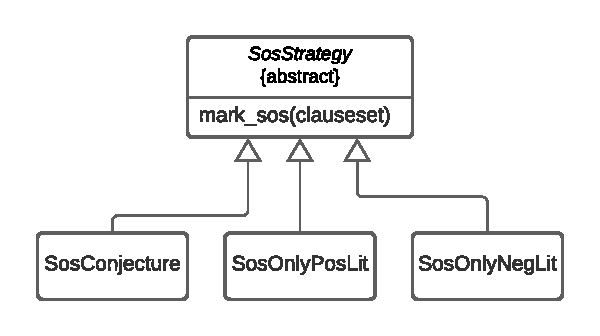
\includegraphics[width=0.7\linewidth]{images/Lucid/SosStrategy0}
	\caption{Klassendiagramm der SOS-Klassen}
	\label{fig:sosstrategy0}
\end{figure}



\section{Anpassung der Beweisprozedur}
\begin{figure}
	\centering
	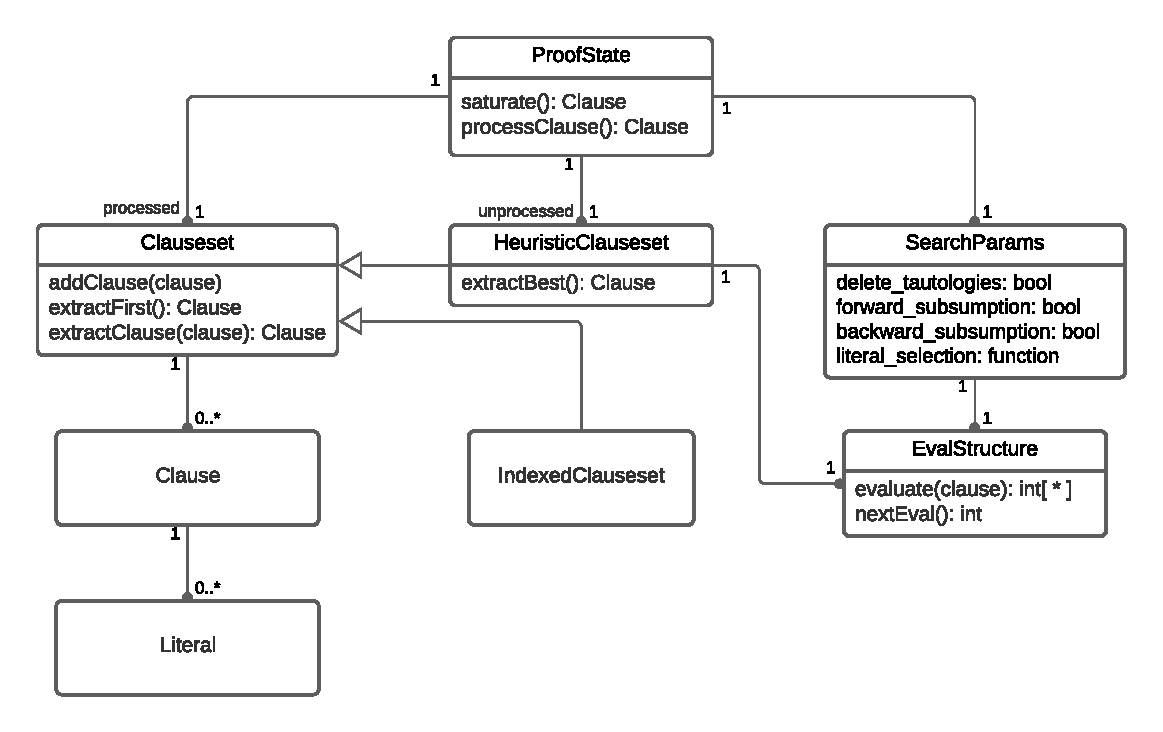
\includegraphics[width=1\linewidth]{images/Lucid/PyResProofState}
	\caption{Klassendiagramm der bisherigen Beweisprozedur}
	\label{fig:pyresproofstate}
\end{figure}

Aufteilungsmöglichkeiten in Grundklauselmenge und SOS, SOS durch Flags in Klauseln darstellen, Strategie, um neue Klausel auszuwählen (Non-SOS in processed, oder alternierend mit Verhältnis),
Sonderfälle: Wenn SOS leer, 